% !Mode:: "TeX:UTF-8"
% !TEX program  = xelatex
\section{Introduction}
% 研究的目的、背景;理论依据、实验基础和研究方法或实验设计;预期结果和意义等
\subsection{Dense Prediction Tasks} 
With the rapid development of computer science research and related industries in recent years, people's production and lifestyle have undergone tremendous changes. Breakthroughs have been made in artificial intelligence, especially in the field of machine learning, and it has also been applied in more and more fields.

Neural networks have made impressive results in a variance of tasks \cite{multivandenhende2021}, such as semantic segmentation \cite{long2015fully}, instance segmentation \cite{he2017mask}, augmented reality \cite{abu2018augmented} and panoptic segmentation \cite{kirillov2019panoptic}. All of them are part of a dense prediction task, a collection of computer vision tasks aiming at labeling every pixel in the given image into a predefined class \cite{huang2021fapn}.


\begin{figure}[htb]
    \centering
    \begin{subfigure}[t]{.45\linewidth}
        \centering
        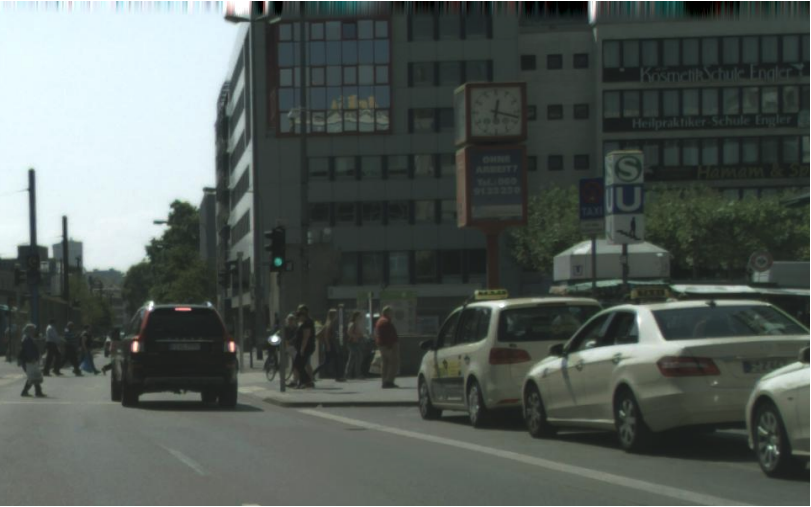
\includegraphics[width=1\textwidth]{figures/RawImage.png}
        \caption{Raw Image}\label{Raw Image}
    \end{subfigure}
    \begin{subfigure}[t]{.45\linewidth}
        \centering
        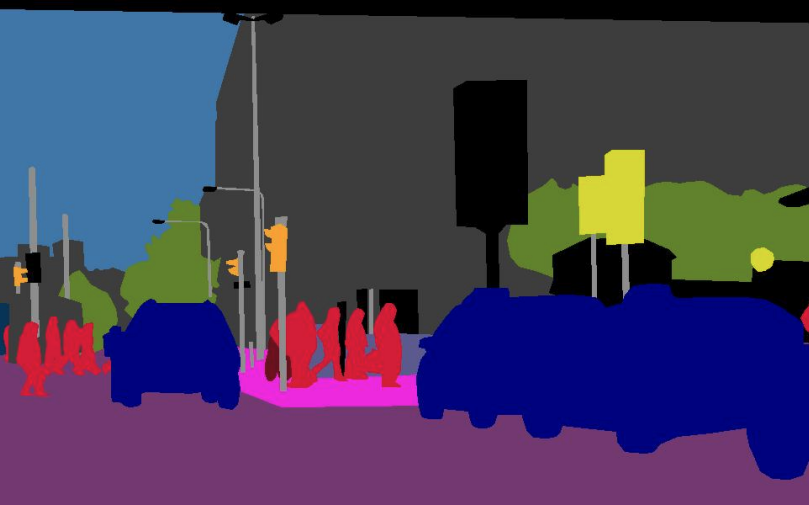
\includegraphics[width=1\textwidth]{figures/Semantic Segmentation2.png}
        \caption{Semantic Segmentation}\label{Semantic Segmentation}
    \end{subfigure}
    \begin{subfigure}[t]{.45\linewidth}
        \centering
        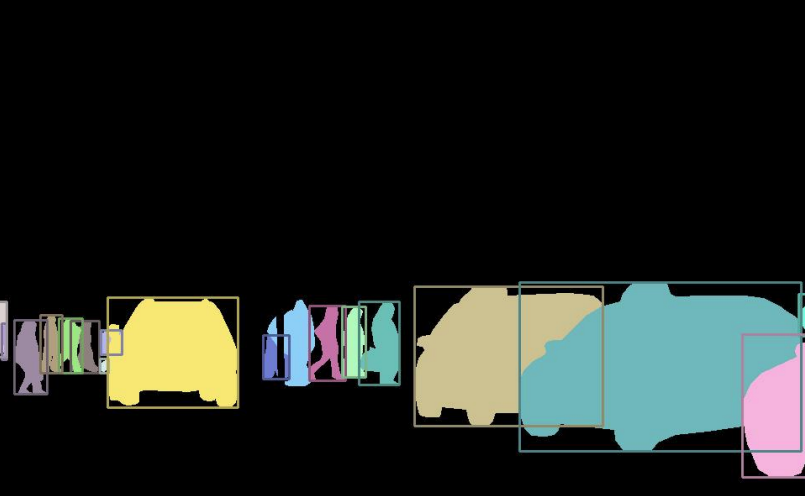
\includegraphics[width=1\textwidth]{figures/Instance Segmentation2.png}
        \caption{Instance Segmentation}\label{Instance Segmentation}
    \end{subfigure}
    \begin{subfigure}[t]{.45\linewidth}
        \centering
        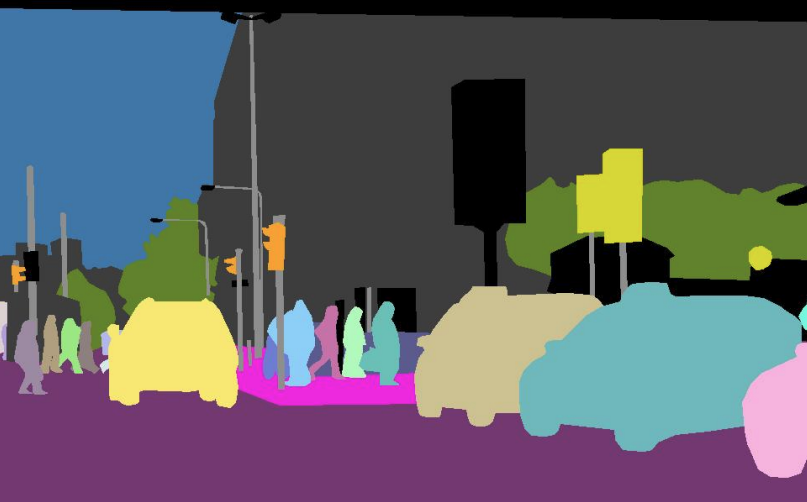
\includegraphics[width=1\textwidth]{figures/PanopticSegmentation.png}
        \caption{Panoptic Segmentation}\label{Panoptic Segmentation}
    \end{subfigure}
    \caption{Computer vision tasks \cite{kirillov2019panoptic}: For a given a) raw image, b) Semantic Segmentation, c) Instance Segmentation, d) Panoptic Segmentation are a part of a dense prediction task, aiming at labeling every pixel in the given image into a predefined class. Panoptic segmentation was proposed by Alexander Kirillov et al. in 2018.}\label{Dense Prediction Tasks}
\end{figure}


Any of these tasks is one of the basic problems of computer vision and has a very high value of use, so it has high importance in various applications, such as autonomous driving \cite{de2017semantic}, medical image segmentation \cite{lei2020medical}, and geospatial object segmentation \cite{zheng2020foreground}.

% Dense prediction可以被视作图像分类任务和目标检测任务的综合任务,其同时需要图像中物体的语义信息和位置信息。为了同时获取两类信息并进行对齐,大多数网络采取了top-down feature pyramid的网络架构。这类网络架构可以获取给定图像不同层级的语义信息;底层网络得到的图像分辨率较高,主要用来获取instance的位置信息;高层图像得到的图像分辨率较低,包含更多抽象的语义信息,用以预测小物体和判断物体边缘的位置。
Dense prediction can be regarded as a comprehensive task of image classification task and object detection task, it needs both semantic information and position information of instances in the given images. To obtain two kinds of information and align them at the same time, most networks adopt the network architecture of the top-down feature pyramid. This type of network architecture can obtain semantic information at different levels of a given image; the image obtained by the lower-level convolution layers has a higher resolution and is mainly used to obtain the location information of the instance; the image obtained by the high-level image has a lower resolution and contains more abstract semantics information for predicting small objects and judging the location of object edges.


\subsection{Research Objectives and Expected Results}
The goal of the graduation project is to reproduce the training process and results of FaPN \cite{huang2021fapn} and apply this high-accuracy dense prediction model on the Jetson Nano, to realize the function of the segment and recognize objects in daily life, such as traffic signs, pedestrian, etc.

In this paper, two methods are applied and deployed on a Jetson Nano to obtain better dense prediction results on the Jetson Nano. The first kind uses the picture on the Jetson Nano through the photo album or camera API, the verified image is then transmitted to the server end for image processing and then re-transmitted back to the front end. Another method is to apply the lightweight paddle-lite \cite{paddlelite} that has been transplanted to the Jetson Nano.

The work of paper can be mainly divided into several parts, including deploying and training the model with and without FaPN and evaluating the difference in the model accuracy, loss, AP, and mIoU to reflect the superiority of FaPN.

Section \uppercase\expandafter{\romannumeral2} \textbf{Related Work}, meanly focus on introducing the main principles and functions of the related modules used and reproduced in this article. This paper gradually understands the structure and innovation of FCN, FPN, FaPN, reproduces the FSM and FAM modules of FaPN.


Section \uppercase\expandafter{\romannumeral3} \textbf{**Undefined**}, 内容未决定


Section \uppercase\expandafter{\romannumeral4} \textbf{Results, Analysis, and Relevant Information}, analyzed training procedure and results. Provides information about training and running environments.


Section \uppercase\expandafter{\romannumeral5} \textbf{Conclusion and Future Work}, summarizes existing work and suggests directions for improvement.
\clearpage